\myChapter{Estensione della libreria FACPL}
\label{cap:estensione_libreria}

Il linguaggio FACPL è basato interamente su una libreria scritta in Java. 
Per implementare la valutazione di richieste basate sul comportamnento passato è stato necessario estendere questa libreria con nuove classi e modificarne alcune.\\ \par
In questo capitolo verranno mostrate le novità introdotte nel capitolo \ref{cap:usagecontrolfacpl} sotto il punto di vista implementativo, per ovvi motivi verranno mostrate solo alcune parti delle modifiche effettuate, ma il codice completo si può comunque trovare su GitHub.

\section{Status e Status Attribute} % (fold)
\label{sec:status_e_status_attribute}
Il primo passo per estendere la libreria è stato la creazione di uno \status, che è modellato da una semplice classe 
di cui ne verrà mostrato un pezzo nel codice~\ref{lst:PezzoStatus1}, successivamente sono stati creati gli \statusattribute.
La relazione che intercorre tra queste nuove classi è mostrata in Figura~\ref{fig:statusUML.png}.
\MyFigure{statusUML.png}{Grafico UML delle classi Status e StatusAttribute}{0.9}
Di seguito invece verranno mostrate queste nuove classi a livello implementativo.
\myIjava{status.java}{Stralcio della classe Status}{1}{15}{PezzoStatus1}
Questa classe ha un campo essenziale per la logica del sistema, ed è una LinkedList di \statusattribute.
In questa classe, oltre ad i costruttori ed alcuni getter sono stati implementati due metodi mostrati in Codice~\ref{lst:PezzoStatus2}, uno per andare a cercare lo \statusattribute, e l'altro per restituirne il valore.
\myIjava{status.java}{Metodi per gli \statusattribute}{22}{32}{PezzoStatus2}
Gli \statusattribute \ sono modellati da una singola classe, anch'essa molto breve e facile da capire.
Come facilmente intuibile dai costruttori in Codice~\ref{lst:costruttoriSA} questa classe ha tre campi, un \texttt{id}, un valore, ed un tipo. 
\myIjava{SA.java}{Costruttori di Status Attribute}{5}{22}{costruttoriSA}
Il senso del secondo costruttore è facilmente intuibile, mentre il primo è stato creato appositamente per dare un valore di default all'attributo nel caso non venisse inizializzato.

% section status_e_status_attribute (end)


\section{Implementazione dei comparatori sugli Status Attribute} % (fold)
\label{sec:implementazione_dei_comparatori_sugli_status_attribute}
Nella libreria di FACPL era già presente una solida struttura (Figura~\ref{fig:comparisonUML.png}), basata su un factory, per la comparazione di attributi, quindi è bastato modificare le varie funzioni in modo tale che potessero operare anche su \statusattribute.
Prendendo in esame la funzione \textit{Equals} vediamo come funziona ora, a livello implementativo, il processo di comparazione.\\ 
\myIjava{equal.java}{Classe che implementa Equal}{1}{29}{equalclass}
Vedendo il codice~\ref{lst:equalclass} si nota che la classe implementa un interfaccia, quest'interfaccia definisce al suo interno un unico metodo astratto, \textit{public Boolean evaluateFunction(List<Object> args)} che sarà il metodo chiamato in fase di valutazione.
La modifica del processo di comparazione è stata fatta in questo metodo, bisognava fare in modo che uno, o entrambi gli argomenti, potessero essere \statusattribute, e per questo è stata introdotta un'altra funzione, chiamata \textit{convertType} che, dato uno \statusattribute, va a ricavarne il valore.\\ \par
Quando verrà richiamato il primo metodo verrà effettuato un controllo sul tipo dell'argomento, e in base a questo risultato verrà chiamato il secondo metodo che effettuerà l'operazione descritta in precedenza.



\begin{sidewaysfigure}
    \centering
	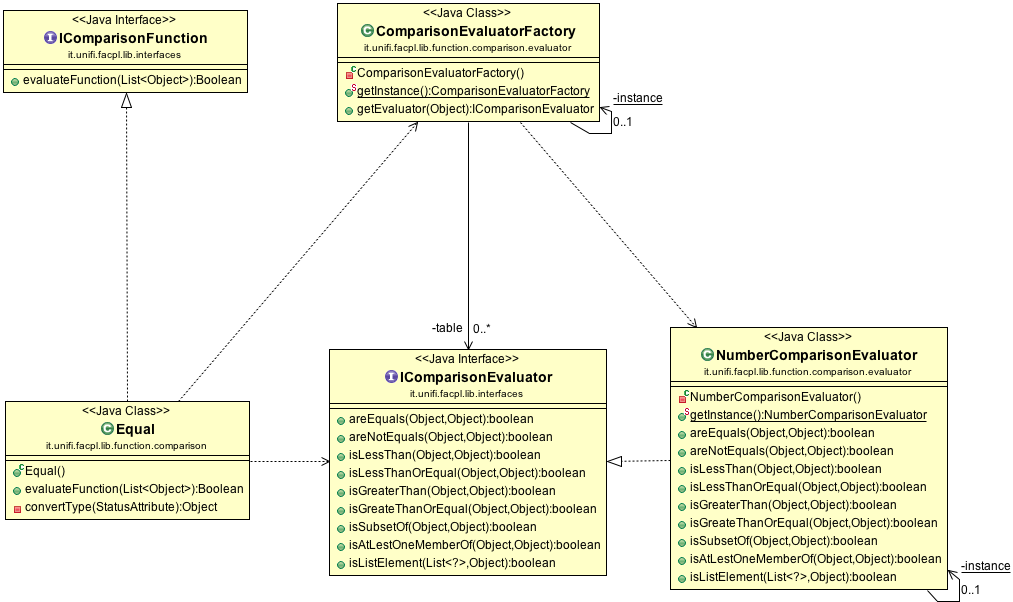
\includegraphics[width=1\linewidth]{comparisonUML.png}
    \caption{Grafico UML per la gerarchia di classi usate nella comparazione}
    \label{fig:comparisonUML.png}
\end{sidewaysfigure}

% section implementazione_dei_comparatori_sugli_status_attribute (end)

\section{Funzioni per la modifica degli Status Attribute} % (fold)
\label{sec:funzioni_aritmetiche_per_la_modifica_degli_statusattribute}
Per concetto di \statusattribute \ è  richiesto dinamismo, in quanto devono irrimediabilmente cambiare rispetto alla valutazione di una richiesta, quindi sono state implementate funzioni che effettuano queste operazioni di modifica.\\ \par
Per mantenere la coerenza con il resto della libreria queste funzioni sono state implementate in modo simile a come sono state implementate quelle di comparazione, motivo per cui l'UML in Figura~\ref{fig:functionarith.png} somiglia molto a quello usato per la comparazione.
Ora verrà mostrato il caso di operazioni numeriche. Sono state implementate anche operazioni su stringhe, ma il funzionamento è analogo alla sua controparte numerica.\\ \par

\begin{sidewaysfigure}
    \centering
	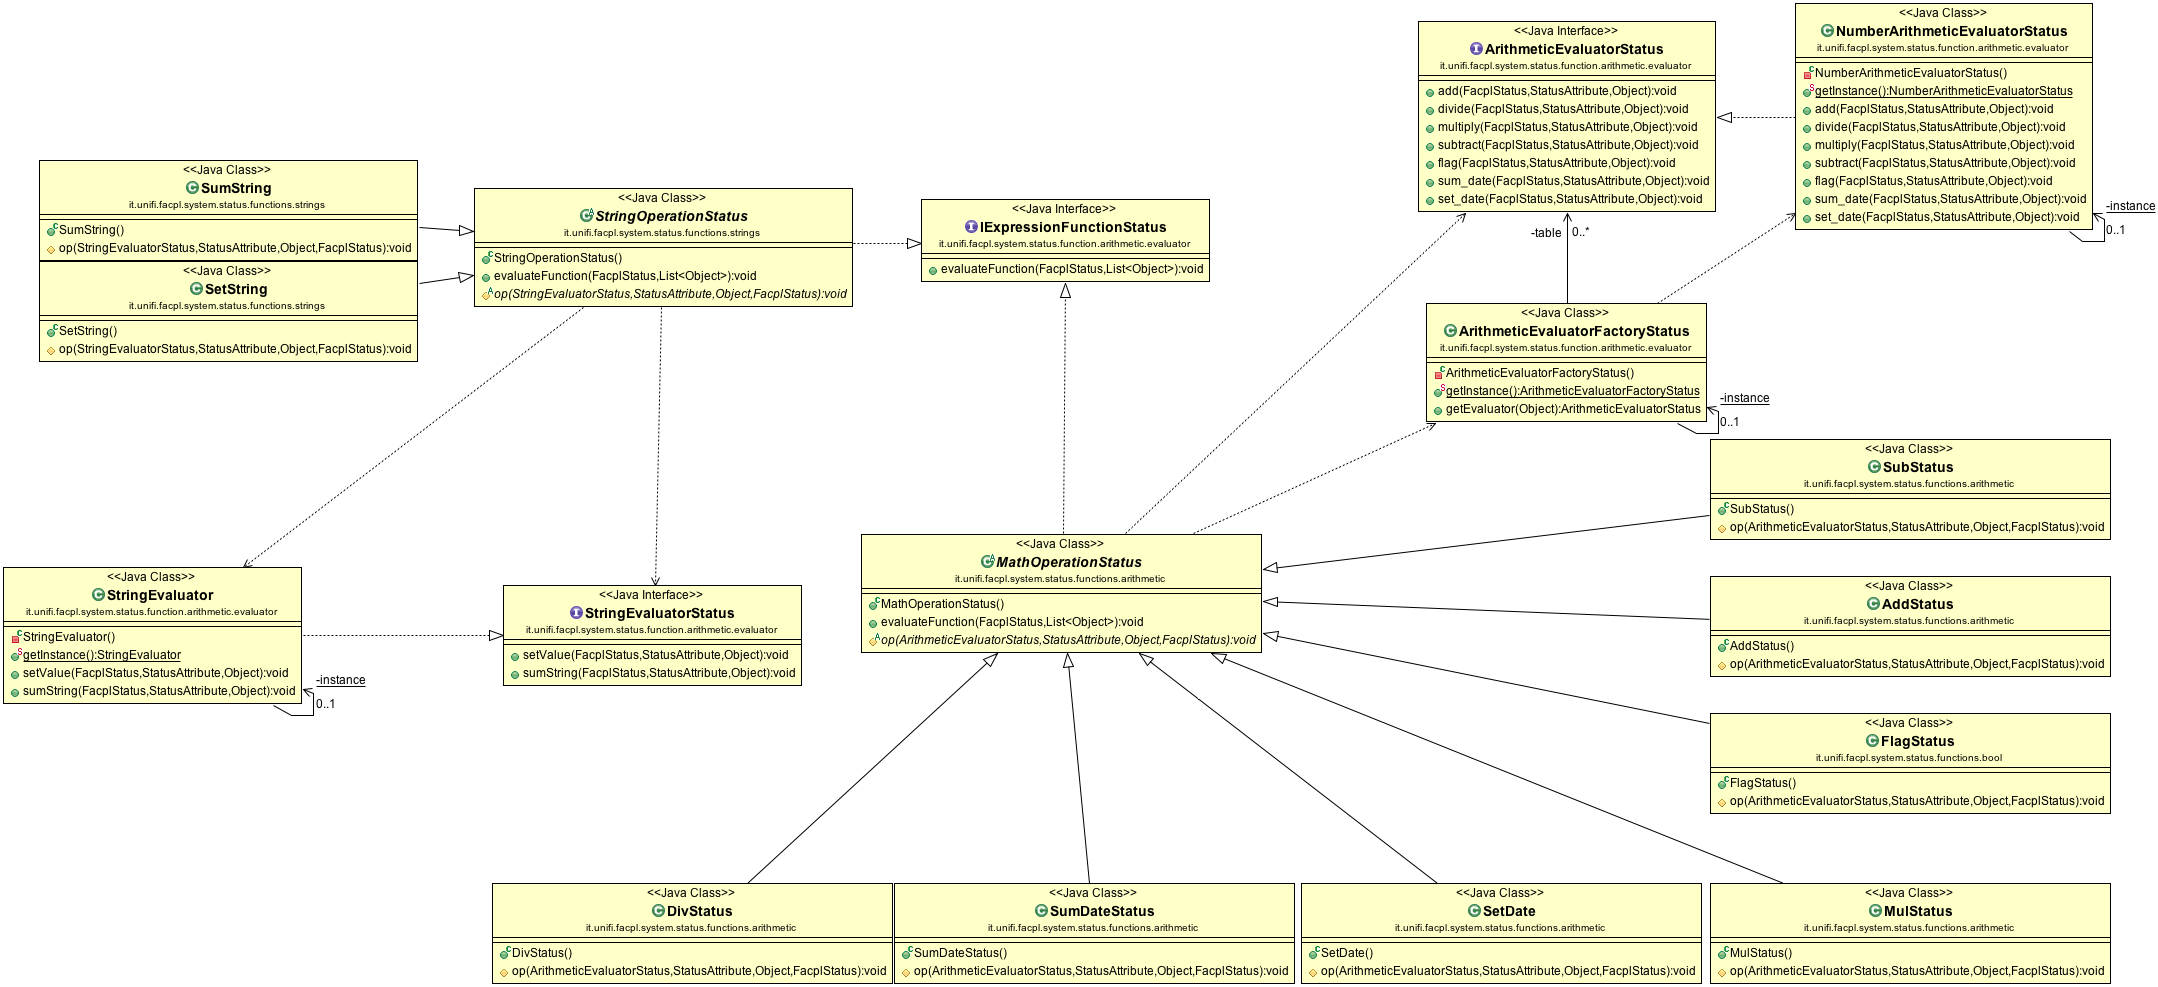
\includegraphics[width=1\linewidth]{functionarith.png}
    \caption{Grafico UML per la gerarchia di funzioni aritmetiche}
    \label{fig:functionarith.png}
\end{sidewaysfigure}

Come si nota dalla Figura~\ref{fig:functionarith.png} tutto parte da un interfaccia, che dovrà essere implementata da tutte le funzioni che andranno a modificare lo stato, quest'ultima è composta da un solo metodo che verrà chiamato per l'esecuzione dell'operazione.
\myjava{IExpressionFunctionStatus.java}{Interfaccia per le operazioni}
In questo caso, da quest'interfaccia deriva una classe astratta per le operazioni aritmetiche che implementerà il metodo astratto dell'interfaccia ed aggiungerà un altro metodo astratto, che rappresenterà la funzione vera e propria.
\myIjava{MathOperationStatus.java}{Metodo implementato dall'interfaccia}{7}{21}{evaluateFunction}
Dal questo codice si notano subito molte somglianze con quello proposto in sezione \ref{sec:implementazione_dei_comparatori_sugli_status_attribute}, questo perché la logica di funzionamento è sostanzialmente la stessa.
Inizialmente viene effettuato un controllo sul tipo degli argomenti, successivamente viene richiesto un valutatore corretto per il tipo di dato passatogli e poi è effettuata l'operazione chiamando il metodo \textit{op}, che sfruttando il principio del pattern Template, è implementato nelle varie sottoclassi differenziando così il comportamento senza dover riscrivere interamente il metodo, risparmiando così molte righe di codice.\\ \par
Le classi che estendono \textit{MathOperationStatus} sono molto simili tra di loro, quindi prenderemo in esame solo la classe che effettua l'operazione di somma, mostrata in basso a sinistra nella Figura~\ref{fig:functionarith.png}.
\myjava{addStatus.java}{Classe per la somma}
Questa classe implementa semplicemente il metodo astratto, chiamando sul valutatore passatogli in precedenza la funzione di somma.\\ \par
Il valutatore non è altro che una classe che implementa tutte le operazioni di una determinata categoria, per esempio in questo caso viene restituito un valutatore che effettua le operazioni aritmetiche.
A puro scopo esemplificativo mostriamo ora come è implementata l'operazione di somma nel valutatore aritmetico.
\myIjava{valutatore.java}{Metodo implementato dall'interfaccia}{27}{39}{valsomma}

\section{Estensione del contesto} % (fold)
\label{sec:estensione_del_contesto}

Lo \status \ creato in \ref{sec:status_e_status_attribute} andrà in qualche modo preso in considerazione durante il processo di valutazione in modo che vada ad influenzare le decisioni.
Di conseguenza lo stato dev'essere inglobato dal contesto in cui viene valutata la richiesta.
\begin{sidewaysfigure}
    \centering
	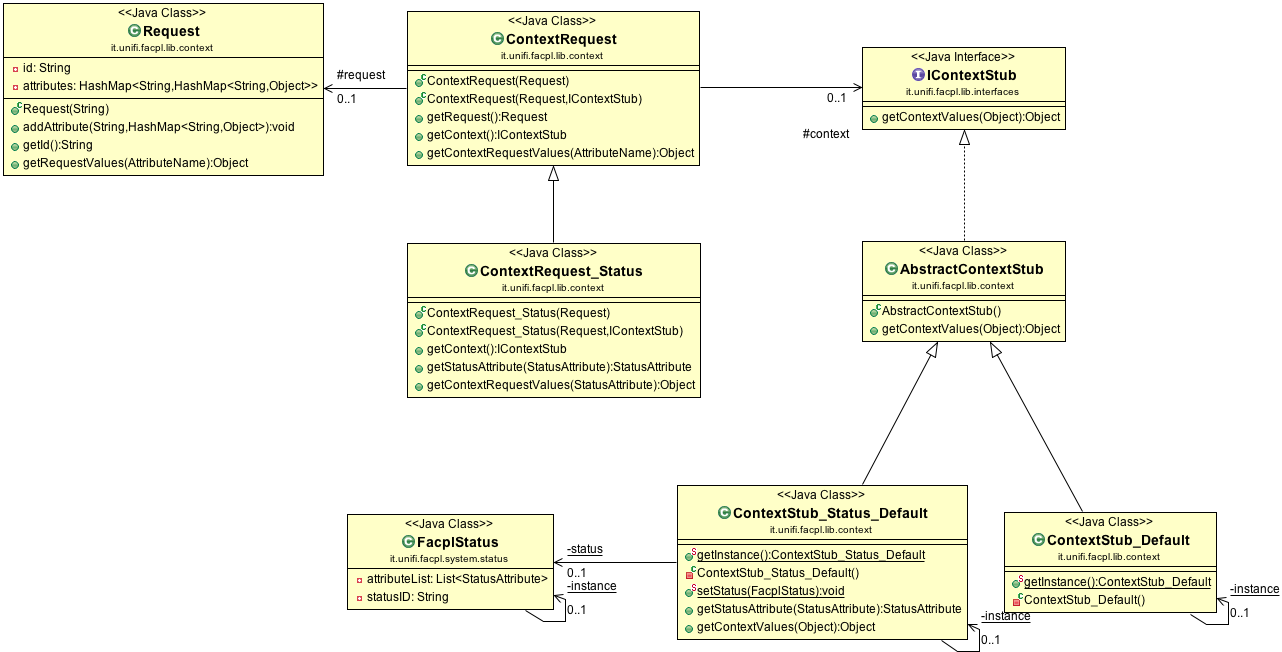
\includegraphics[width=1\linewidth]{context.png}
    \caption{Grafico UML del contesto}
    \label{fig:context.png}
\end{sidewaysfigure}

Per prima cosa è stato necessario estendere la gerarchia di classi derivanti dall'interfaccia \textit{IContextStub}. Come si può vedere in figura \ref{fig:context.png} è stata fatta un'operazione di refactoring astraendo alcune parti in comune, ed è stata creata la classe \textit{ContextStub\_Default\_Status} di cui ora ne verrà analizzata l'implementazione.\\ \par
Come si nota dall'immagine \ref{fig:context.png} la classe è implementata come un \textit{Singleton} e contiene diversi metodi legati a \status, uno di questi è il \textit{Setter}, che permette di aggiungere lo stato, l'altro invece è un \textit{Getter} che permette di ricavare un attributo dallo stato.
Il metodo più importante invece è quello mostrato in Codice~\ref{lst:getterstub}
\myIjava{stubstatus.java}{Classe ContextStub\_Default\_Status}{17}{28}{getterstub}
Questo metodo permette di effettuare la ricerca mostrata in figura \ref{fig:evalStatus}, ovvero datogli un attributo andrà prima a verificare la sua presenza all'interno dello \status, dopodiché se non lo trova verificherà la presenza all'interno dell'ambiente.\\ \par
Successivamente è stata estesa anche alla classe \textit{ContextRequest} con una nuova classe \textit{ContextRequest\_Status}, la cui unica differenza è un semplice \textit{Getter} per gli attributi di stato.

\section{Obligations e PEP} % (fold)
\label{sec:obligations_e_pep}

Lo stato alla necessità andrà aggiornato, e qua entrano in gioco due componenti fondamentali del sistema, il PEP e le \textit{Obligations}. 

\begin{sidewaysfigure}
    \centering
	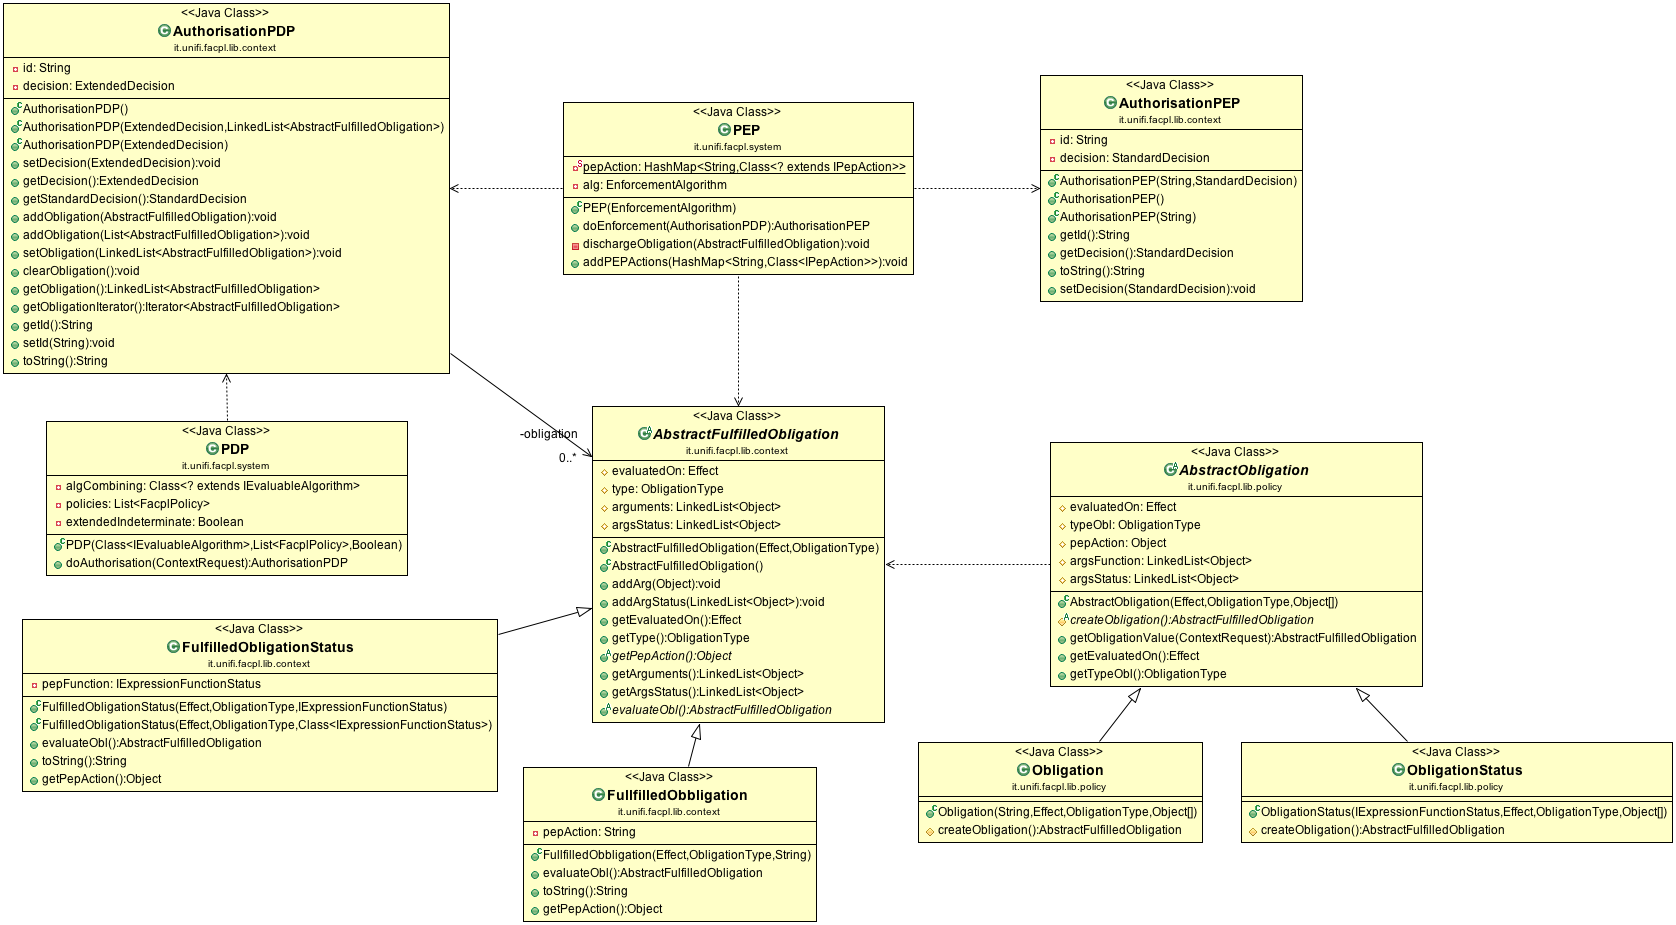
\includegraphics[width=1\linewidth]{obl.png}
    \caption{Relazioni tra Obligation e PEP}
    \label{fig:obl.png}
\end{sidewaysfigure}


Anche in questo caso sono state estese le \textit{Obligation} introducendo un nuovo tipo chiamato \textit{Obligation Status}, questo tipo particolare di \textit{Obligation} servono per andare ad eseguire azioni sullo stato.
Nel sistema sono presenti due tipo fondamentali di \textit{Obligation}, il primo sono quelle a livello sintattico, le seconde, chiamate \textit{FulfilledObligations} sono quelle pronte ad essere valutate. Vediamo adesso come sono state estese quelle a livello sintattico.\\ \par
Per eseguire questa estensione è stato reso necessario un refactoring, per prima cosa è stato astratto tutto il comportamento comune in una superclasse astratta, successivamente è stata creata la nuova classe che modella questo nuovo tipo.
Il refactoring ha coinvolto anche il metodo che si occupa del \textit{Fulfilling} delle \textit{Obligation} in quanto ora deve creare anche questo nuovo tipo, la scelta più ovvia è stata creare un metodo astratto implementato nelle due sottoclassi che viene chiamato dalla superclasse per creare il tipo corretto.
\myIjava{absObl.java}{Parte rifattorizzata del metodo che si occupa del fulfilling}{16}{18}{fulfilabs}
\myIjava{oblStat.java}{CreateObligation nelle status}{17}{24}{createoblstat}
\myIjava{oblNorm.java}{CreateObligation nelle normali}{11}{14}{createoblnorm}
La \textit{Obligation} di stato necessiterà anche di argomenti su cui eseguire l'azione, che le verranno passati in fase di costruzione.\\ \par
Alla fine della valutazione il PDP crea un oggetto di tipo \textit{AuthorisationPDP} che conterrà la decisione e una lista di \textit{FulfilledObligation}, quest'ultime poi andranno al PEP per la loro valutazione. Vediamo ora come sono state implementate.\\ \par
Anche in questo caso è stato necessario un refactoring analogo a quello fatto per le prime.
\myIjava{FulOblStat.java}{Peculiarità della classe FulfilledObligationStatus}{1}{15}{pecfulstat}
Come si può notare, in fase di costruzione, gli verrà passato un oggetto di tipo \textit{IExpressionFunctionStatus} che sarà l'azione che andrà a eseguire sullo stato. Quest'azione andrà realmente ad essere eseguita quando verrà chiamato dal PEP il metodo \textit{evaluateObl}.\\ \par
Il PEP nella fase di enforcement effettua la valutazione delle \textit{Obligation}, in questo caso le modifiche per permettere al sistema di eseguirle sono state minime, è bastato modificare il metodo \textit{DischargeObligation} in modo che quando gli viene passata una \textit{AbstractFulfilledObligation} chiamasse il metodo \textit{evaluateObl} .
\myIjava{PEP.java}{Discharge delle Fulfilled Obligation di stato}{102}{106}{PEP}
% section obligations_e_pep (end)


\section{Plugin di Eclipse} % (fold)
\label{sec:plugin_eclipse}
[TODO: CORREGGERE PARTE SU XTEND E MAGARI ALLUNGARE]
Il progetto è basato su Java, ed il codice formalizzato in FACPL viene successivamente convertito in codice Java attraverso un processo di autogenerazione.
Per fare questo si usa un linguaggio chiamato XTend.
\MyFigure{xtendLogo.png}{Logo di Xtend}{0.35}
XTend ha le sue radici in Java, ma si concentra maggiormente su aspetti come una sintassi più concisa, ed altre funzionalità come l'inferenza sui tipi, l'overload degli operatori o l'estensione dei metodi (?). 
È principalmente un linguaggio \textit{Object-oriented}, ma integra caratteristiche tipiche di un linguaggio funzionale, come ad esempio le Lambda Expression. Il sistema dei tipi di XTend è lo stesso di Java, ed è quindi statico.\\ \par

\section{Esempio}
\label{sec:esempio}

In questa sezione verrà mostrato come sarà in Java il corrispettivo del Codice \ref{lst:PrimoEsempio_FACPL} e del Codice \ref{lst:PrimoEsempioRichieste_FACPL}.\\ \par
Tutto parte dalla classe dove è presente il metodo Main (Codice~\ref{lst:mainprimoesempio.java}. In questo stesso modulo viene preparato il sistema all'esecuzione attraverso l'inizializzazione di tutti i componenti necessari al sistema.\\ \par
I due componenti più importanti sono il PDP e il PEP che vengono inizializazati nel costruttore, in quest'ultimo vengono anche aggiunte le \textit{Policy} e creato un contesto. Successivamente all'inizializzazione verranno inserite tutte le richieste in una lista e partirà un ciclo che effettuerà l'operazione di autorizzazione del PDP e di enforcement del PEP.
\myjava{mainprimoesempio.java}{Main di uno scenario FACPL}
Per esigienze di comodità il contesto è stato integrato in un'unica classe insieme alle richieste.
\myjava{esempiocontesto.java}{Richiesta e contesto}
Il metodo che si occupa della creazione dello stato è \textit{createStatus()}, il quale non farà altro che crearsi una serie di attributi ed inseririrli in un nuovo oggetto di tipo \textit{FacplStatus}, per poi restituirlo.
La richiesta invece viene restituita sottoforma di un oggetto di tipo \textit{ContextRequest\_Status}, il quale verrà restituto dal primo dei due metodi. La richiesta è formata da diverse \textit{Hashmap} che sono come le categorie degli attributi che verranno inseriti al loro interno.
Queste hashmap poi vengono aggiunte ad un oggetto \textit{Request} insieme ad una stringa che racchiude l'informazione riguardante la categoria dell'oggetto appena inserito.
Alice, in Codice \ref{lst:PrimoEsempioRichieste_FACPL}, richiede ad un certo punto un'azione identificata come \textit{(action / id , "stopRead")}, ed insieme a questo attributo manderà anche altri due attributi, uno che rappresenta il suo nome, e l'altro che contiene il nome del file su cui deve essere effettuata l'azione. L'attributo riguardante l'azione viene codificato alle righe 11 e 15.\\ \par
Come ultima cosa vediamo come viene codificato un set di \textit{Policy}. Come detto in precedenza una \textit{Policy} è formata da un \textit{Target}, eventualmente altre \textit{Policy} o \textit{Rule} e delle \textit{Obligation}. Prendiamo ora in esempio una \textit{Policy} che contiene tutti e tre questi elementi.
\myIjava{richiestajavaprimoesempio.java}{Policy StopRead}{92}{122}{polstopread}
In particolare è stata presa in considerazione la \textit{Policy} che permette di fermare la lettura, ovvero quella che verrà valutata quando verrà effettuata la richiesta in Codice \ref{lst:esempiocontesto.java}.\\ \par
Tutte le \textit{Policy} derivano da una classe astratta che verrà estesa secondo le necessità. Come detto prima questa \textit{Policy} contiene tutti e tre gli elementi che la caratterizzano, in particolare la \textit{Obligation} che in questo caso è una \textit{ObligationStatus}. Questa \textit{Obligation} viene aggiunta come tutte le altre, ovvero chiamando l'apposito metodo della superclasse, ed è costruita passandogli come parametro un'azione da effettuare e gli argomenti, in questo caso l'azione è la sottrazione e gli argomenti è l'attributo che rappresenta il numero di lettori e l'intero 1. \\ \par
\myIjava{richiestajavaprimoesempio.java}{Expression Function che valuta un attributo di stato}{42}{45}{expressionfunctstat}
Nel Codice \ref{lst:expressionfunctstat} si può vedere come una \textit{ExpressionFunction} riesca a valutare un attributo di stato.


% section esempio (end)
    

